
\chapter{Etapy przetwarzania danych szkolnych}
\textit{Katarzyna Śmietanka} \\
Przystosowanie algorytmów do realnych danych uzyskanych z jednej ze szkoł ponadgimnazjalnych wymagało przeprowadzenia procesu eksploracji danych, czyli przetworzenia danych oraz wyodrębnienia istotnych danych dla zdefiniowanego przez nas problemu. Na proces obróbki danych składało się kilka etapów: analiza danych, wybór istotnych danych, transformacje danych, czyszczenie i uzupełnienie brakujących danych oraz stworzenie wizualizacji danych.
\section{Opis danych szkolnych}
Uzyskane dane szkolne są plikami tekstowymi w formacie CSV. \\
W sekcji tej poniższe pojęcia będą używane synonimicznie: \\
kurs - przedmiot \\
program nauczania - klasa \\
Rodzaje plików z danymi:
\begin{enumerate}
\item[1.] Dla każdej klasy nauczane przedmioty oraz uczący nauczyciele.
\begin{verbatim}
Format:
<Nazwa przedmiotu><Prowadzący przedmiot>
\end{verbatim}
\item[2.] Grupy występujace w szkole
\begin{verbatim}
Format:
<Kod grupy> <Grupa nadrzędna> <Nazwa grupy> <Rodzaj grupy> 
<Opiekun grupy><Liczba uczniów><Rok szkolny><Status grupy>
<Inkrementować numer><Osoba wprowadzająca><Data wprowadzenia>
\end{verbatim}
\item[3.] Słownik godzin lekcyjnych
\begin{verbatim}
Format:
<ID>	<Nazwa><Godzina rozpoczęcia><Godzina zakończenia><Aktywny>
\end{verbatim}
\item[4.] Lista miejsc
\begin{verbatim}
Format:
<ID><Miejsce><Aktywny>
\end{verbatim}
\item[5.] Zestawienie planu
\begin{verbatim}
Format:
<Plan zajęć><Rok szkolny><Grupa uczniów><Cykl><Data zajęć>
<Okres cyklu od><Okres cyklu do><Termin><Godzina lekcyjna>
<Godzina rozpoczęcia> <Godzina zakończenia><Zajęcia><Miejsce><Prowadzący>
\end{verbatim}
\end{enumerate}
\section{Etapy przetwarzania danych}
\begin{figure}[H]
  \centering
    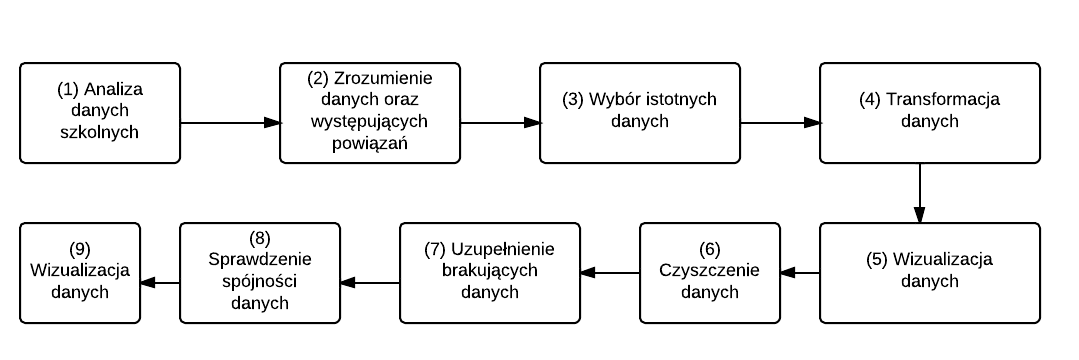
\includegraphics[width=0.8\textwidth]{proces_przetwarzania.png}
  \caption{Szkip etapów przetwarzania danych}
\end{figure}
\begin{enumerate}
\item[(1)] \textbf{Analiza danych szkolnych} - zapoznanie się z danymi oraz analiza w jaki sposób efektywnie i racjonalnie wykorzystać nagromadzoną wiedzę, poznanie struktury danych.
\item[(2)] \textbf{Zrozumienie danych oraz identyfikacja występujących powiązań} - szczegółowe poznanie zależności pomiędzy poszczególnymi danymi występującymi m.in. grupami uczniów a klasami, przedmiotami a nauczycielami prowadzącymi zajęcia.
\item[(3)] \textbf{Wybór istotnych danych} - wyodrębnienie istotnych danych niezbędnych do stworzenia wykonywalnego planu zajęć: klasy, przedmioty, które są nauczane w danej klasie, liczba uczniów uczestniczących w danych zajęciach, informacje o przedmiotach międzyklasowych, liczbie godzin realizowanego przedmiotu oraz prowadzących dany przedmiot.
\item[(4)] \textbf{Transformacja danych} - wykonane transformacje opisane w sekcji ,,Transformacje''
\item[(5)] \textbf{Wizualizacja danych} - wykonanie grafów przedstawiających zależności pomiędzy danymi, szczegółowy opis w sekcji ,,Wizualizacja danych szkolnych''
\item[(6)] \textbf{Czyszczenie danych}  - usunięcie niepełnych, niepoprawnych oraz nieistotnych danych np. kursy (przedmioty), które mają niepełne dane zaburzające działanie algorytmu, usunięcie zbędnych kursów m.in. $Biblioteka\ szkolna$, który w znacznym stopniu utrudniał ułożenie planu poprzez zwiększenie liczby konfliktów pomiędzy zajęciami.
\item[(7)] \textbf{Uzupełnienie brakujących danych} - dane uzyskane ze szkoły nie zawierały informacji o maksymalnej liczbie osób, która może się zmieścić w danej sali, typach sal szkolnych - co jest dość istotnym elementem, który wpływa na realność ułożonego planu. Nie uzwględnienie tego czynnika może powodować, że np. zajęcia z matematyki będą musiały odbywać się na sali gimnastycznej. 
\item[(8)] \textbf{Sprawdzenie spójności danych} - wczytanie danych do struktury początkowej dla zaimplementowanych algorytmów.
\item[(9)] \textbf{Wizualizacja danych} - w celu łatwiejszej identyfikacji występujących błędów oraz sprecyzowanie trudności ułożenia planu zajęć dla tych danych.
\end{enumerate}
\subsection{Transformacje}
Przetworzenie danych szkolnych do formatu konkursowego wymagało przeprowadzenia kilku transformacji danych, które zostały wymienione poniżej:
\begin{enumerate}
\item Odczytanie istniejących grup w szkole i przypisanie tych grup do poszczególnych klas, wyodrębnienie klas na podstawie \verb#<Grupa nadrzędna> <Nazwa grupy>#
\item Identyfikacja grup międzyklasowych z dokumentu ,, Zestawienie planu'' przy pomocy funkcji \verb#groupby()# \cite{groupby} na podstawie wspólnych kluczy: 
\begin{verbatim}
<Termin><Godzina lekcyjna><Zajęcia>
	<Godzina rozpoczęcia><Godzina zakończenia><Prowadzący>
\end{verbatim}
Po reformie oświaty w szkołach ponadgimnazjalnych uczniowie uzyskali możliwość wyboru nauczanych przedmiotów na poziomie rozszerzonym, co spowodowało powstanie grup międzyklasowych realizujących ten sam przedmiot. \\
Jako, że grupy międzyklasowe nie posiadały jednego wspólnego identyfikatora, który był taki dla sam dla kilku klas, konieczne było przeprowadzenie operacji grupowania. \\
Przykład:
\begin{verbatim}
Dane z dokumentu "Zestawienie planu":
>>>2013/2014 Wrzesień;2013/2014 aktywny;2 LW Chemia;Tygodniowy;;
	2013-09-16;2014-01-31;Poniedziałek;Lekcja 1;08:00;08:45;
	Chemia CHEM;Sala 119;ŚaAa
>>>2013/2014 Wrzesień;2013/2014 aktywny;2 LP Chemia;Tygodniowy;;
	2013-09-16;2014-01-31;Poniedziałek;Lekcja 1;08:00;08:45;
	Chemia CHEM;Sala 119;ŚaAa
Występujące identyfikatory grup: 
2 LW Chemia
2 LP Chemia
\end{verbatim}
Pomimo różnych identyfikatorów można zauwazyć, że  grupy \verb#2 LW Chemia# oraz 
\verb#2 LP Chemia# tworzą jedną z grup międzyklasowych, ponieważ są nauczane przez tego samego nauczyciela oraz odbywają się dokładnie w tym samym czasie.
\item Przypisanie identyfikatorów grup międzyklasowych do odpowiednich klas (stworzenie międzyklasowych kursów), dla których dany przedmiot jest nauczany. Zliczenie liczby godzin realizowanego kursu międzyklasowego i liczby studentów uczęszczających na dany kurs.
\item Wyodrębnienie wszystkich przedmiotów nauczanych w szkole (nauczanych tylko w obrębie jednej klasy) oraz przypisanie ich do opowiednich klas.
\item Zgrupowanie danych z dokumentu ,,Zestawienie planu'' na podstawie kluczy: \\
\verb#<Zajęcia><Grupa uczniów># w celu zliczenia liczby godzin realizowanego przedmiotu w danej klasie oraz przypisania identyfikora nauczyciela. \\
Dokument ,,Zestawienie planu'' zawiera aktualnie ułożony plan szkolny, w którym każde zajęcia przyporządkowane są do dnia tygodnia i godziny lekcyjnej oraz klasy. Aby uzyskać liczbę godzin nauczanego przedmiotu lub liczbę uczniów, konieczne było przeprowadzenie operacji grupowania.
\end{enumerate}
\subsection{Specyfikacja uzyskanych danych}
\begin{table}[H]
\begin{center}

\begin{tabular}{ |c|c|c| }
\multicolumn{1}{r}{}
 &  \multicolumn{1}{c}{$$}
 & \multicolumn{1}{c}{$$} 
 \\
\cline{1-2}
$Liczba\ przedmiotów\ (kursów)$ & $373$\\
\cline{1-2}
$Liczba\ klas\ (programów\ nauczania)$ & $22$\\
\cline{1-2}
$Liczba\ dni$ & $5$ \\
\cline{1-2}
$Licza\ przedziałów\ czasowych$ & $15$ \\
\cline{1-2}
$Liczba\ ograniczeń$ & $0$ \\
\cline{1-2}
\end{tabular}
\end{center}
\caption {Opis przetworzonych danych}
\end{table}
Dla przypadku testowego ,,Dane szkolne'' nie zostały wprowadzone żadne ograniczenia, ponadto rozszerzono $Licza\ przedziałów\ czasowych$ z $11$ na $15$. \\
Uzasadnienie rozszerzenia liczby przedziałów czasowych: \\
Zaimplementowane przez nas algorytmy nie uwzględniają możliwości przydzielenia zajęć, które należącą do tego samego programu nauczania, do jednakowego przedziału czasowego w planie zajęć. Co w obecnej specyfikacji problemu byłoby jednoznaczne z naruszeniem ograniczeń twardych\\
Przykład wyjaśniający problem dla klasy o identyfikatorze \verb#2 LW#:
\begin{verbatim}
Do programu nauczania dla tej klas należą kursy:
2 LW WF Dziewczęta
2 LW WF Chłopcy
\end{verbatim}
Osoba układająca plan posiada wiedzę, które zajęcia będące w programie nauczania dla danej klasy mogą odbywać się w tym samym czasie. Konieczne jest tu sprawdzenie czy zbiory uczęszczających uczniów na te zajęcia są rozłączne oraz nauczane są przez innego nauczyciela. \\
Z uzyskanych danych nie jesteśmy w stanie jednoznacznie wywnioskować rozłączności zbiorów, choć intuicyjnie wydaje się to oczywiste dla przypadku przedmiotu: $Wychowanie\ fizyczne$, że grupy uczniów uczęszczających na zajęcia  \verb#2 LW WF Dziewczęta# i \verb#2 LW WF Chłopcy# są zbiorami rozłącznymi.
Mniej intuicyjny przykład dla klasy o identyfikatorze \verb#1 4A#:
\begin{verbatim}
Do programu nauczania dla tej klasy należą kursy:
1 4A Warsztaty A
1 4A Warsztaty B
1 4A Warsztaty C
1 4A Warsztaty D
\end{verbatim} 
Prawdopodobnie klasa podzielona jest na 4 rozłączne grupy albo na 2 różne grupy, a każdy uczeń należy do dwóch z czterech grup. Precyzyjne stwierdzenie wymagałoby szczegółowej konsultacji z osobami układającymi plan w szkole. \\
Dlatego też zdecydowaliśmy się na uproszczenie problemu, poprzez przyporządkowanie wszystkich grup należących do danej klasy, w wyniku czego zajęcia dla każdej z grup muszą odbywać się w różnym czasie, stąd wynika konieczność rozszerzenia przedziałów czasowych. 
\subsection{Wizualizacje danych szkolnych}
\par Poniższe grafy zostały stworzone przy pomocy biblioteki JavaScript, D3.js. Wierzchołki oznaczają kursy (przedmioty) zaś krawędzie w grafie konflikty pomiędzy kursami. Konflikty pomiędzy kursami występują, kiedy dany kurs należy do tego samego programu nauczania co kurs połączony z nim bezpośrednio krawędzią, bądź oba kursy prowadzone są przez tego samego wykładowcę.
Zajęcia połączone krawędzią nie mogą być przeprowadzane w tym samym czasie. 
\par Stworzenie wizualizacji danych dało możliwość obejrzenia struktury danych wejściowych, sprawdzenia ich poprawności oraz identyfikację nieprawidłowych zależności pomiędzy kursami. Naniesienie wszystkich organiczeń na graf dało bardzo nieczytelną strukturę grafu, dlatego też zdecydowano się na rozdzielenie poszczególnych ograniczeń i przedstawienie uzyskanych zależności pomiędzy kursami.
\begin{figure}[H]
  \centering
  \caption{Fragment grafu przedstawiający konflikty pomiędzy pomiędzy kursami, uwzględniając zależności związane z tym samym prowadzącym zajęcia. Grafy pełne.}
    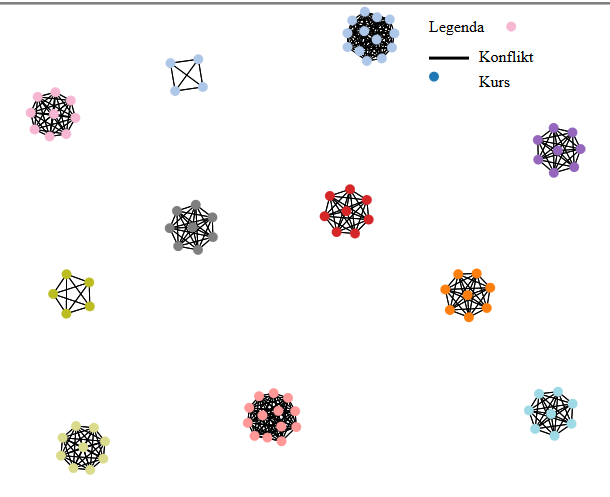
\includegraphics[width=10cm]{szkola1.PNG}
\end{figure}
\par Graf pokazuje konflikty pomiędzy zajęciami, po uwzględnieniu ograniczeń dotyczących tego samego prowadzącego nauczyciela, który uczy w kilku grupach przedmiotowych. Uzyskana struktura grafu jest prawiłowa, ponieważ w danym czasie nauczyciel jest w stanie prowadzić zajęcia tylko w jednej grupie przedmiotowej. Na wizualizację składają się grafy pełne zawierające wszystkie zależności dotyczące konfliktów uwzględniających tego samego wykładowcę.
\begin{figure}[H]
  \centering
   \caption{Fragment grafu przedstawiający grupy konfliktujących ze sobą kursów ze względu na należenie do tych samych programów nauczania}
   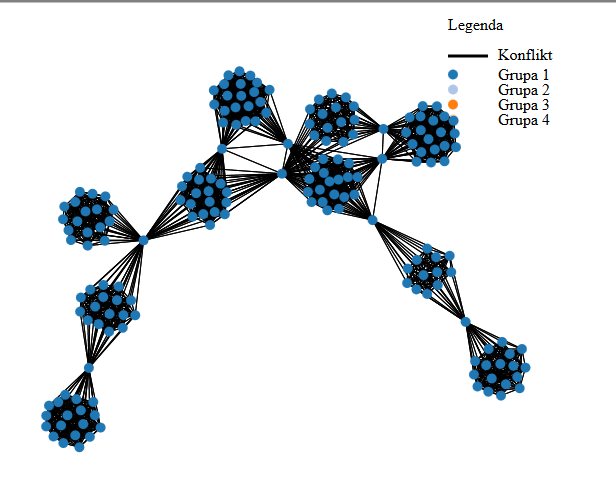
\includegraphics[width=10cm]{fragmentszkola.PNG}
\end{figure}
\par Na grafie została pokazana część zależności pomiędzy kursami uwzględniając ograniczenie dotyczące tylko przynależenia kursów do tego samego programu nauczania. Zagnieżdżone grupy kursów reprezentują programy nauczania, zaś wierzchołki łączące te grupy są to zajęcia międzyklasowe.

\subsection{Implementacja}
Projekt został napisany w Python 2.7 \\
Wizualizacje zostały stworzone z wykorzystaniem biblioteki JavaScript D3.js \cite{wiz}
\section{Trudności w analizie i przetwarzaniu danych}
\begin{enumerate}
\item \textbf{Nadmiarowość danych} - po wstępnej analizie okazało się, że część z uzyskanych danych nie jest potrzeba do wyodrębniania istotnych dla algorytmów danych. Uzyskane pliki z danymi zawierające informacje o przedmiotach nauczanych w każdej klasie i nauczycielach prowadzących okazały się być zbędne. W tych danych nie było dołączonej informacji o liczbie godzin realizowanego przedmiotu ani liczbie uczniów uczęszczających na ten przedmiot. 
\item \textbf{Niespójność konwencji nazewnictwa w danych} - utrudniało to w znacznym stopniu analizę danych i powiązań pomiędzy występującymi grupami wchodzącymi w skład klasy. Grupy międzyklasowe mimo tego, że miały dokładnie te same zajęcia w tym samym czasiem i prowadzone były przez tego samego nauczyciela, identyfikatory tych grup były różne dla każdej z klas.
\item \textbf{Niepełne i czasami niepoprawne dane} - brak danych o nauczycielu uczącym danego przedmiotu, brak informacji o liczbie osób uczęszczających na dane zajęcia. Niepełne dane powodowały błędne działanie algorytmu. Uzupełnienie brakujących danych domyślnymi danymi wprowadzało kolejne konflikty pomiędzy kursami, które znacznie utrudniały oraz modyfikowały problem ułożenia planu dla tej szkoły.
\item \textbf{Integracja danych} - konieczność łączenia danych w celu wyodrębnienia informacji o poszczególnych przedmiotach i grupach uczniów. W celu uzyskania danych niezbędnych do specyfikacji problemu koniecznym było połączenie danych z kilku plików, dotyczy to głównie grup międzyklasowych, które występują dla tej szkoły.
\item \textbf{Odtworzenie danych} - konieczność odtworzenia niektórych danych z istniejącego planu zajęć dla szkoły zdefiniowanego pliku ,,Zestawienie planu''. Dane nie zawierały ściśle określonej liczby godzin realizowanego przedmiotu przez daną klasę, dlatego też trzeba było to uzyskać, zliczając poszczególne wystąpienia zajęć w istniejącym planie ułożonym przez szkołę.
\item \textbf{Dostosowanie danych do formatu} - dostosowanie danych szkolnych do formatu zdefiniowanego w danych konkursowych. Narzucony ściśle format danych wejściowych znacznie utrudniał problem przetworzenia danych, gdyż związane było to koniecznością zdefiniowania poszczególnych zajęć, w szczególności zajęć międzyklasowych w zadanej konwencji przez organizatorów konkursu.
\item \textbf{Brakujące dane} - uzupełnienie brakujących danych (typ sali, w jakim typie sali mogą odbywać się zajęcia z danego przedmiotu, wielkość sali).  Dane nie zawierały istotnej informacji o pojemności sali oraz typie sali. Dane te zostały uzupełnione po konsultacji z osobą pracującą w tej szkole i posiadającą wiedzę na ten temat.
\end{enumerate}


